\documentclass[12pt]{article}
\usepackage[a4paper]{geometry}
\usepackage[utf8]{inputenc}
\usepackage{url}
\usepackage{hyperref}
\usepackage[french]{babel}
\usepackage[T1]{fontenc}
\usepackage{graphicx}
\usepackage{tgheros}
\usepackage{listings}
\usepackage{forest}
\renewcommand{\familydefault}{\sfdefault}

\lstset
{ 
    language=xml,
    basicstyle=\footnotesize,
    numbers=left,
    stepnumber=1,
    showstringspaces=false,
    tabsize=4,
    breaklines=true,
    breakatwhitespace=false,
}

\title{Rapport Projet Tuteuré Rundeck}
\author{HEPPNER Tristan / ROYER Grégory
\\
TORRES Yanis / AISSI Ayoub }
\date{Janvier 2020}

\begin{document}

\maketitle
\newpage
\tableofcontents
\newpage
\section{Remerciements}

Nous remercions notre tuteur de projet tutoré, Mr Fabien PASCALE, Expert en calcul scientifique au CNRS, pour nous avoir fait découvrir Rundeck, ses enjeux ainsi que l'ampleur et l'importance de ce projet.
\vspace{0.5cm}
\\
Merci  à  Monsieur Lucas  Nussbaum,  Debian  Project  Leader  (DPL),  maître  de conférences à l'Université de Lorraine et chercheur auprès du laboratoire LORIA, pour nous avoir permit de nous enrichir intellectuellement.
\vspace{0.5cm}
\\
Que cette licence ASRALL(Administration de Systèmes, Réseaux et Applications à base  de  Logiciels  Libres)  puisse  perdurer  dans  le  temps,  et  toujours  apporter  les connaissances indispensables dont nous, les élèves et futurs administrateurs, avons besoin. Un grand merci à Monsieur Philippe Dosch, enseignant et responsable de la licence, qui a su, quand il le fallait, nous écouter et nous donner les indications nous permettant de prendre la bonne direction.
\newpage
\section{Introduction}
Depuis l’apparition de l’Homme sur la terre, ce dernier n’a eu de cesse que de trouver divers moyens pour améliorer la vie de ses semblables. Nous sommes,  par  nature, des  êtres sociables, sociaux et dotés d’intelligence. 
\\
L'Homme, étant doté d'intelligence et de créativité 

\section{Sujet de la soutenance}

La finalité de ce projet est de proposer une solution permettant d'automatiser la gestion d'un parc informatique grâce à une seule et unique machine.

Pour cela, nous allons analyser les solutions existantes :
\begin{itemize}
    \item Rundeck
    \item Jenkins
    \item Buildbot
    \item Ansible Tower
    \item JobScheduler
    \item Crontab
\end{itemize}
\vspace{0.5cm}
L'objectif de ce projet, est quant à lui de démontrer l'utilité de la solution Rundeck.
\vspace{0.5cm}
\\
A la fin du projet, nous disposerons :
\begin{itemize}
    \item Tutoriel de mise en place de Rundeck
    \item Comparaison des solutions existantes
\end{itemize}
\vspace{0.5cm}
\textbf{Tuteur du projet : }
\\
PASCALE Fabien \hspace{3.3cm} fabien.pacale@gmail.com
\vspace{0.5cm}
\\
\textbf{Étudiants : }
\\
AISSI Ayoub \hspace{4.2cm} aa.w-a@hotmail.fr
\\ 
HEPPNER Tristan \hspace{3.2cm} tristan.heppner@outlook.com
\\ 
ROYER Grégory \hspace{3.5cm} gregory.royer@hotmail.com
\\ 
TORRES Yanis \hspace{3.7cm} yanis.torres@outlook.com
\\
\vspace{0.5cm}
\\
Avant de débuter l'analyse des solutions, une définition du mot \textbf{Automatisation} est de rigueur afin de pouvoir aborder, dans les meilleurs conditions possibles, ce sujet.
\\
Nous allons ensuite analyser chaque solution avec un bref historique, son contexte d'utilisation, la présentation de la solution, son fonctionnement, ses fonctionnalités ainsi qu'un bref conclusion sur cette solution.
\\
Nous aborderons ensuite la solution choisit avec un tutoriel sur sa mise en place.

\section{L'automatisation}

\textit{Déf : L’automatique est une science qui traite de la modélisation, de l’analyse, de l’identification et de la commande des systèmes dynamiques.}
\vspace{0.5cm}
\\
Dans le monde que nous connaissons, on peut voir, sans s'en rendre compte, un quantité astronomique de systèmes automatiques. En effet, l'automatisation d'un système est une chose à laquelle l'homme ne cesse de penser. 
\\
L'automatisation est une science très ancienne datant de l'Antiquité. Dans l'antiquité Romaine, le  niveau de l'eau qui transitait sur les aqueducs était réguler par des valves.
\\
Depuis, l'Homme n'a jamais cessé d'automatiser les éléments qui l'entoure. De célèbre invention ont vu le jour telles que le régulateur à boules de James Watt en 1769.
\\
La science de l'automatique n'a renoncer d'évoluer et de gagner en popularité
\\
L'automatisation, telle que nous l'a connaissons aujourd'hui est devenue fondamentale dans certains domaines notamment dans l'industrie ou encore les systèmes informatiques.

\section{Principes d'automatisations}

L'automatisation d'un parc informatique consiste à diminuer le nombre de tâches d'un administrateur en automatisant certains processus.
\\
Un administrateur système est responsable de chaque machine présente dans un parc et par conséquent sur un réseau.
\\
Le responsable du parc est régulièrement confronté à des tâches récurrents notamment pour les mises à jours de systèmes et/ou logiciels
\\
L'automatisation permet d'effectuer les tâches sans que l'administrateur ai besoin de faire ces tâches sur chaque machine, une à une.
\\
En termes de tâches redondantes, on peut retrouver les sauvegardes du système, les arrêts automatique des machines sur une plage horaire définie, le nettoyage des logs etc...
\\
L'objectif de l'automatisation d'un ou plusieurs systèmes est de pouvoir faire gagner en productivité, en temps de travailler mais aussi de pouvoir réduire les coûts.

\section{Rundeck}

\begin{figure}[ht]
    
\includegraphics[scale=0.8]{images/rundeck.jpg}
    \caption{Logo de Rundeck}
\end{figure}

\subsection{Présentation}

Rundeck est un logiciel Open-Source d'automatisation de gestion de parc informatique. Rundeck est définit comme un orchestrateur de tâches. 
\\
Sorti en 2011, il dispose d'une variante entreprise appelé "Rundeck Entreprise" permettant la gestion d'un parc informatique de plus grande envergure. 
\\
Rundeck est également un logiciel cross-platform disponible pour les systèmes UNIX, Windows et Mac OS. 
\\
Rundeck est hébergé sur la plate forme de développement GitHub, ce qui permet à chaque utilisateur de Rundeck de contribuer à son développement. 
\\
Rundeck est en majeur partie, amélioré grâce à ses utilisateurs. Ces derniers peuvent participer au développement de Rundeck par la notification de bugs/fonctionnalités manquantes ou en rejoignant une équipe de développement de Rundeck. 
\\
Rundeck est développé en JAVA et propose une interface WEB (requiert les paquets JAVA), une interface CLI (Command-Line Interface) ainsi qu'une API REST.

\subsection{Historique et versions}

Rundeck est apparu en 2011 suite à la demande de plus en plus forte du besoin de pouvoir administrer tous les serveurs d'un parc informatique depuis un seul serveur d'administration central. La dernière version en date est la version 3.2.0 datant du 10 février 2020.

\subsection{Contexte d'utilisation}

Rundeck est, parmi un large panel de logiciel d'automatisation, un des plus utilisé lorsque l'utilisateur souhaite automatiser la gestion d'un parc informatique depuis une seule machine physique.

\subsection{Fonctionnement}

Rundeck permet l'exécution de tâches et/ou jobs sur des serveurs distant via une connexion SSH. Rundeck fonctionne sur des réseaux privées où les machines possèdent des adresses IP statiques. 
\\
Les adresses IP dynamique des serveurs distants peuvent causer des conflits d'IP et de clés SSH sur le serveur de Rundeck.
\\
Rundeck également basé sur le principe maître/esclave (master/slave) : La machine où se trouve l'application Rundeck est le maître tandis que le serveur distant est l'esclave. 
\\
De plus, Rundeck montrera un meilleur fonctionnement si celui-ci est installé sur une distribution orientée serveur telles que CentOS. Par défaut, Rundeck écoute sur le port 4440 (http) mais peut également écouté sur le port 4443 (https)
\\
Cependant, Rundeck peut être installé sur d'autres distributions telles qu'Ubuntu, Debian ou même Windows à la seule conditions d'avoir les paquets Java correspondants sous peine de rencontrer des problèmes d'exécution ou d'affichage.
\\
Rundeck, par défaut, fonctionne avec sa propre base de données, un interface WEB ainsi qu'un compte administrateur dont les identifiants sont "admin" pour le nom d'utilisateur et "admin" pour le mot de passe

\subsection{Fonctionnalités}

Rundeck possède une grande gamme de fonctionnalités qui permettent à l'utilisateur de Rundeck, une gestion optimale d'un parc informatique. Rundeck mets à disposition un choix de plus de 1000 plugins de nature diverses et variées. 
\\
Rundeck propose également diverses fonctionnalités notamment l'exécution de commandes/taches à distances
\\
Rundeck également très modulable. En effet, Rundeck utilise un base de données pour l'enregistrement de données telles que les jobs, les clés SSH, les utilisateurs qui ont accès à Rundeck.

\subsection{Conclusions}

\section{Jenkins}

\begin{figure}[ht]
    
\includegraphics[scale=0.5]{images/jenkins.png}
    \caption{Logo de Jenkins}
\end{figure}

\subsection{Présentation}

Jenkins est un logiciel Open-Source d'automatisation, tout comme Rundeck
\\
Sorti en 2011, Jenkins est un dérivé de son prédécesseur Hudson.
\\
Jenkins est également un logiciel cross-platform disponible sur les systèmes UNIX, Windows et Mac OS. 
\\
Jenkins est hébergé sur la plate forme GitHub, ce qui permet à chaque utilisateur de Rundeck de contribuer à son développement. 
\\
Jenkins est en majeur partie, amélioré grâce à ses utilisateurs. Ces derniers peuvent participer au développement de Rundeck par la notification de bugs/fonctionnalités manquantes ou en rejoignant une équipe de développement de Rundeck. 
\\
Rundeck est développé en JAVA et propose une interface WEB et requiert donc des dépendances JAVA.

\subsection{Historique et versions}

Tout comme Rundeck, Jenkins sort en 2011 et est également disponible sur la plate forme GitHub.
\\
Sa dernière version en date est la 2.204.1 datant du 18 décembre 2019.
\\
Jenkins apparaît suite à la cessation d'Hudson par Oracle à la fondation Eclipse. Jenkins devint en 2011, le successeur d'Hudson.
\\
Contrairement à Jenkins, Hudson est un framework d'intégration automatique.

\subsection{Contexte d'utilisation}

Jenkins est un logiciel d'intégration continu utilisé pour la compilation automatique de code source lors de la création de nouveaux programmes et/ou mises à jours .

\subsection{Fonctionnement}

Jenkins est une application WEB en JAVA et se déploie de manière autonome dans un conteneur WEB de type Tomcat.
\\
Cependant, Jenkins peut fonctionner sur toutes les plates-formes pouvant exécuter une JVM (JAVA Virtual Machine) parmi lesquelles on retrouve Ubuntu/Debian, Windows ou même Mac OS à la seule conditions d'avoir les paquets Java correspondants sous peine de rencontrer des problèmes d'exécution ou d'affichage.
\\
Jenkins exécute de manière continue la construction des projets ou "build".
\\ 
Afin que Jenkins puisse permettre l'intégration continue, 
\\
Jenkins exécute les directives de fabrication du logiciel (compilation, assemblage, tests, packaging, ...).
\\
De la même manière que Rundeck, Jenkins peut exécuter des jobs, soit sur lui-même, soit sur des serveurs distants.
\\
Les jobs constituant les builds peuvent être exécutés sur le serveur Jenkins lui-même ou répartis sur plusieurs machines distantes. Jenkins conserve l'historique de toutes les exécutions des jobs et peut notifier par mail ou par RSS en cas erreur.

\subsection{Fonctionnalités}
\subsection{Conclusions}

\section{Buildbot}

\begin{figure}[ht]
    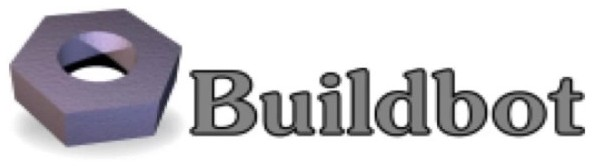
\includegraphics[scale=0.7]{images/buildbot.jpg}
    \caption{Logo de Buildbot}
\end{figure}

\subsection{Présentation}
Tout comme Jenkins, Buildbot est un logiciel Open-Source d'automatisation
\\
Buildbot est un logiciel cross-platform et est disponible sur les systèmes Windows et POSIX (Portable Operating System Interface)
\\
Ce logiciel est présentée comme un alternative au projet de Mozilla : \underline{Tindebox}
\\
Buildbot se démarque de ses concurrents notamment grâce à sa légèreté ainsi que la possibilité de l'installer sur des systèmes d'exploitations portables. En effet, en terme de légèreté, ce programme ne pèse que 4.6MB.
\subsection{Historique et versions}
La première version de Buildbot est sortie le 26 avril 2003. Sa dernière est la 2.0.7 et est daté du 27 février 2020.
\subsection{Contexte d'utilisation}
Buildbot est utilisé dans le cadre de la compilation automatique de "builds". De grandes entreprises, telles que Mozilla, Chromium, WebKit et bien d'autres, utilisent Buildbot.
\subsection{Fonctionnement}
\subsection{Fonctionnalités}
\subsection{Conclusions}

\section{Ansible Tower}

\begin{figure}[ht]
    
\includegraphics[scale=0.4]{images/ansible_tower.png}
    \caption{Logo d'Ansible Tower}
\end{figure}

\subsection{Présentation}
\subsection{Historique et versions}
\subsection{Contexte d'utilisation}
\subsection{Fonctionnement}
\subsection{Fonctionnalités}
\subsection{Conclusions}

\section{JobScheduler}

\begin{figure}[ht]
    \centering
    
\includegraphics[scale=0.6]{images/jobscheduler.jpg}
    \caption{Logo de JobScheduler}
\end{figure}

\subsection{Présentation}
JobSchecduler est un ordannanceur en Open-Source .
\subsection{Historique et versions}
\subsection{Contexte d'utilisation}
\subsection{Fonctionnement}
\subsection{Fonctionnalités}
\subsection{Conclusions}

\section{Cron}

\begin{figure}[ht]
    
\includegraphics[scale=0.5]{images/crontab.png}
    \caption{Logo de Crontab}
\end{figure}

\subsection{Présentation}

\textit{Cron est la troncation de crontab, lui-même la troncation de chrono table qui signifie « table de planification »}
\\
Cron est un fonctionnalité native des systèmes Unix. C'est un planifiateur de tâches
\subsection{Historique et versions}
\subsection{Contexte d'utilisation}
\subsection{Fonctionnement}
\subsection{Fonctionnalités}
\subsection{Conclusions}

\section{Mise en place de Rundeck}
\subsection{Environnement de travail}
\subsection{Installation}
\subsubsection{Exigences système}

\begin{itemize}
    \item Linux: Distributions récentes conseillées pour un fonctionnement optimal
    \item Windows : XP, Server et supérieures (Distributions récentes conseillées)
    \item Mac : OS X 10.4 ou supérieure
\end{itemize}

\vspace{0.5cm}

Accès root (ou administrateur) non requis; création d'un compte utilisateur dédié créer conseillé par Rundeck 

\vspace{0.5cm}

\textbf{Informations complémentaires fournies par Rundeck}
\begin{itemize}
    \item OS supportés :  Red Hat Enterprise Linux - CentOS - Ubuntu - Windows Server
    \item Dernière versions supportés de Mozilla Firefox ou Google Chrome (les autres navigateurs peuvent fonctionner mais présentant des problèmes d'affichage)
    \item 2 CPU
    \item 4 GB de mémoire RAM minimum
    \item 20 GB d'espace disques minimum
    \item Base de données supportées : MySQL - MariaDB - PostgreSQL - Oracle
    \item Logs : Système de fichiers
\end{itemize}

\vspace{0.5cm}

La version 1.8 de JAVA est également requise
\subsubsection{Windows}

\subsubsection{Linux}

L'installation de Rundeck sous Linux est très simpliste. Afin d'obtenir un fonctionnement optimal, Rundeck a été mis en place sous CentOS. Son installation s'est composé des étapes suivantes : 

\vspace{0.5cm}

\begin{itemize}
    \item sudo yum -y install java-1.8.0-openjdk java-1.8.0-openjdk-devel -y \# Installation de la version de Java requise
    \item sudo rpm -Uvh http://repo.rundeck.org/latest.rpm \# Récupération de la dernière version de Rundeck
    \item sudo yum -y install rundeck \# Installation de Rundeck
\end{itemize}

\subsection{Configuration}
\subsubsection{Arborescence}
Les fichiers de configurations de Rundeck sont répartis de manière à pouvoir se repérer dans sa configuration, c'est-à-dire, les fichiers de configuration de Rundeck sont stockés dans le répertoire /etc/rundeck tandis que les fichiers de configurations propres aux tâches/jobs, est stockés dans le répertoire /var/lib/rundeck. 
\\
Ci-dessous, la disposition DEB/RPM :
\newpage
\begin{forest}
  for tree={
    font=\ttfamily,
    grow'=0,
    child anchor=west,
    parent anchor=south,
    anchor=west,
    calign=first,
    edge path={
      \noexpand\path [draw, \forestoption{edge}]
      (!u.south west) +(7.5pt,0) |- node[fill,inner sep=1.25pt] {} (.child anchor)\forestoption{edge label};
    },
    before typesetting nodes={
      if n=1
        {insert before={[,phantom]}}
        {}
    },
    fit=band,
    before computing xy={l=15pt},
  }
[/etc/rundeck/
  [admin.aclpolicy]
  [apitoken.aclpolicy]
  [artifact-repositories.yaml]
  [cli-log4j.properties]
  [framework.properties]
  [jaas-loginmodule.conf]
  [profile]
  [project.properties]
  [realm.properties]
  [rundeck-config.properties]
  [rundeckpro-licence.key]
  [ssl 
    [ssl.properties]
    [keystore]
    [truststore]
  ]
  [system-job\_reader\.aclpolicy\_template]
  [system-job\_runner\.aclpolicy\_template]
  [system-job\_viewer\.aclpolicy\_template]
  [system-job\_writer\.aclpolicy\_template]
  [system-project\_admin\.aclpolicy\_template]
]
\end{forest}

\newpage

\begin{forest}
  for tree={
    font=\ttfamily,
    grow'=0,
    child anchor=west,
    parent anchor=south,
    anchor=west,
    calign=first,
    edge path={
      \noexpand\path [draw, \forestoption{edge}]
      (!u.south west) +(7.5pt,0) |- node[fill,inner sep=1.25pt] {} (.child anchor)\forestoption{edge label};
    },
    before typesetting nodes={
      if n=1
        {insert before={[,phantom]}}
        {}
    },
    fit=band,
    before computing xy={l=15pt},
  }
  [/var/lib/rundeck
  [bootstrap]
  [cli]
  [data]
  [libext]
  [logs]
  [projects]
  [repository]
  [var]
  [work]
]
\end{forest}
\vspace{0.5cm}
\\
Ci-dessous, la disposition de l'interface de Rundeck :
\vspace{0.5cm}
\\
\vspace{0.5cm}
\begin{forest}
  for tree={
    font=\ttfamily,
    grow'=0,
    child anchor=west,
    parent anchor=south,
    anchor=west,
    calign=first,
    edge path={
      \noexpand\path [draw, \forestoption{edge}]
      (!u.south west) +(7.5pt,0) |- node[fill,inner sep=1.25pt] {} (.child anchor)\forestoption{edge label};
    },
    before typesetting nodes={
      if n=1
        {insert before={[,phantom]}}
        {}
    },
    fit=band,
    before computing xy={l=15pt},
  }
  [\$RDECK\_BASE/etc/
  [admin.acmpolicy]
  [apitoken.aclpolicy]
  [cli-log4j.properties]
  [framework.properties]
  [preferences.properties]
  [profile]
  [profile.bat]
  [project.properties]
]
\end{forest}
\\
\vspace{0.5cm}
\begin{forest}
  for tree={
    font=\ttfamily,
    grow'=0,
    child anchor=west,
    parent anchor=south,
    anchor=west,
    calign=first,
    edge path={
      \noexpand\path [draw, \forestoption{edge}]
      (!u.south west) +(7.5pt,0) |- node[fill,inner sep=1.25pt] {} (.child anchor)\forestoption{edge label};
    },
    before typesetting nodes={
      if n=1
        {insert before={[,phantom]}}
        {}
    },
    fit=band,
    before computing xy={l=15pt},
  }
  [\$RDECK\_BASE/server/config/
  [artifact-repositories.yaml]
  [jaas-loginmodule.conf]
  [log4j.properties]
  [realm.properties]
  [rundeck-config.properties]
  [ssl.properties]
]
\end{forest}
\\
\vspace{0.5cm}
\\
Dans le cadre de notre projet, nous avons appliqué une configuration simple, impliquant les fichiers de configurations suivants :
\begin{itemize}
    \item /etc/rundeck/framework.properties
    \item /etc/rundeck/realm.properties
    \item /etc/rundeck/rundeck-conf.properties
\end{itemize}
\vspace{0.5cm}
\textbf{Informations sur les fichiers utilisés :}
\\
\textit{framework.properties :} Fichier de configuration utilisé par les services de base de Rundeck
\\
\textit{rundeck-conf.properties :} Fichier de configuration de l'application WEB
\\
\textit{realm.properties :} Fichier de configuration des propriétés des utilisateurs

\subsubsection{URL d'accès}
Rundeck est fourni, par défaut, avec une interface web dont l'URL est : 
\\
\underline{\url{http://localhost:4440}}
\vspace{0.2cm}
\\
Cette URL peut, toutefois être modifié, en éditant les fichiers \textit{framework.properties} et \textit{rundeck-config.properties}.
\\
Le paramètre \textit{framework.rundeck.url} contient l'URL de base de Rundeck et peut être remplacé par une adresse au choix

\subsubsection{Définition de la méthode de stockage}

Selon les choix de l'administrateur de Rundeck, plusieurs méthodes de stockages sont à disposition.

Méthode de stockage :
\begin{itemize}
    \item Base de données embarquée
    \item Base de données "personnelle"
    \item Système de fichiers
\end{itemize}

\subsubsection{Définition des nodes}
Un node permet d'ajouter un serveur, une machine que l'on souhaite automatiser avec Rundeck.
\\
Les nodes sont définis, communément, dans un fichier au format XML mais peuvent également être définis dans un fichier au format YAML et JSON. Cette définition doit suivre une syntaxe imposé par Rundeck. On peut définir autant de nodes que l'on souhaite dans ce fichier.
\vspace{0.5cm}
\\
\textit{Ces exemples sont à titres indicatifs et sont fournis dans la documentation de Rundeck}
\vspace{0.5cm}
\\
Ci-dessous, la déclaration d'un node dans Rundeck, crée par l'utilisateur au format \textbf{XML}
\vspace{0.5cm}
\\
\begin{lstlisting}
<?xml version="1.0" encoding="UTF-8"?>

<project>
  <node name="localhost" 
        description="Rundeck server node" 
        tags="" 
        hostname="localhost" 
        osArch="amd64" 
        osFamily="unix" 
        osName="Linux" 
        osVersion="2.6.21.7-2.fc8xen" 
        username="rundeck"/>
</project>
\end{lstlisting}

\vspace{0.5cm}
Ci-dessous, la déclaration d'un node dans Rundeck, crée par l'utilisateur au format \textbf{JSON}
\vspace{0.5cm}
\\

\begin{lstlisting}
{
  "madmartigan.local": {
    "tags": "local,server",
    "osFamily": "unix",
    "username": "greg",
    "osVersion": "10.10.3",
    "osArch": "x86_64",
    "description": "Rundeck server node",
    "hostname": "madmartigan.local",
    "nodename": "madmartigan.local",
    "osName": "Mac OS X"
  },
  "test": {
    "tags": "alphabet, soup",
    "osFamily": "unix",
    "ssh-key-storage-path": "keys/testkey1.pem",
    "username": "vagrant",
    "osVersion": "10.10.3",
    "osArch": "x86_64",
    "description": "Rundeck server node",
    "hostname": "192.168.33.12",
    "nodename": "test",
    "osName": "Mac OS X"
  }
}
\end{lstlisting}

\vspace{0.5cm}
Ci-dessous, la déclaration d'un node dans Rundeck, crée par l'utilisateur au format \textbf{YAML}
\vspace{0.5cm}
\\

\begin{lstlisting}
Venkman.local:
  description: Rundeck server node
  hostname: Venkman.local
  nodename: Venkman.local
  osArch: x86_64
  osFamily: unix
  osName: Mac OS X
  osVersion: 10.6.6
  tags: ''
  username: greg
\end{lstlisting}

\vspace{0.5cm}
Cette configuration est identique pour chaque ordinateur/serveur que l'on souhaite automatiser.
\vspace{0.5cm}
\\
\textbf{Informations sur la syntaxe}
\begin{itemize}
    \item name : nom de l'ordinateur/serveur (obligatoire)
    \item description : brève description du node (facultatif)
    \item tags : nom permettant l'identification du node (facultatif)
    \item hostname : adresse IP de la machine (obligatoire)
    \item osArch : Architecture du système (facultatif)
    \item osFamily : Famille du système (facultatif)
    \item osName : Nom du système (facultatif)
    \item osVersion : Version de l'OS (facultatif)
    \item username : compte avec lequel rundeck se connecte à la machine distante (obligatoire)
\end{itemize}
\vspace{0.5cm}
La définition d'un node dans le format YAML ou JSON diffère légèrement du format XML.
\subsubsection{Clés SSH}
Rundeck requiert les clés SSH de chaque machine qu'il a sous son contrôle

\subsubsection{Définition des jobs}
Un job est décomposé en plusieurs "step"

\subsection{Utilisation}
\subsubsection{Pilotage de service}
\subsubsection{Création de jobs}
La création d'un job peut être fait directement sur l'interface Rundeck. 
\\
Rundeck propose également à l'utilisateur de pouvoir exécuter un script provenant d'un site web externe, ou même de pouvoir exécuter un script déjà écrit à l'avance. 

\newpage
\section{Bibliographie}

\begin{itemize}
    \item \url{https://docs.rundeck.com/docs/administration/install/}
    \item \url{https://docs.rundeck.com/docs/manual/}
    \item \url{http://docs.buildbot.net/current/index.html}
    \item \url{https://github.com/rundeck/rundeck}
    \item \url{https://docs.rundeck.com/docs/administration/configuration/config-file-reference.html}
    \item \url{https://tech.oyster.com/rundeck-vs-crontab-why-rundeck-won/}
    \item \url{https://www.edureka.co/blog/what-is-jenkins/}
\end{itemize}

\newpage
\section{Annexes}

\end{document}
